%
% wavelets.tex -- Wavelets auf Graphen
%
% (c) 2020 Prof Dr Andreas Müller, Hochschule Rapperswil
%
\section{Wavelets auf Graphen
\label{buch:section:wavelets-auf-graphen}}
\rhead{Wavelets auf Graphen}
Graphen werden oft verwendet um geometrische Objekte zu approximieren.
Funktionen auf einem Graphen können dann Approximationen von physikalischen
Grössen wie zum Beispiel der Temperatur auf dem geometrischen Objekt
interpretiert werden.
Verschiedene Basen für die Beschreibung solcher Funktionen sind im Laufe
der Zeit verwendet worden, doch Wavelets auf einem Graphen sind eine
neuere Idee, mit der man aus der Laplace-Matrix Basen gewinnen kann,
die die Idee von langsam sich ausbreitenden Störungen besonders gut
wiederzugeben in der Lage sind.

In diesem Abschnitt werden erst Funktionen auf einem Graphen genauer
definiert.
In Abschnitt~\ref{buch:subsection:standardbasis-und-eigenbasis}
wird die Eigenbasis mit dem Laplace-Operator konstruiert und mit
der Standarbasis verglichen.
Schliesslich werden in Abschnitt~\ref{buch:subsection:wavelet-basen}
verschiedene Wavelet-Basen konstruiert.

\subsection{Funktionen auf einem Graphen und die Laplace-Matrix}
Sei $G$ ein Graph mit der Knotenmenge $V$.
Eine Funktion $f$ auf einem Graphen ist eine Funktion $f\colon V\to\mathbb{R}$.
Funktionen auf $G$ sind also Vektoren, die mit den Knoten $V$ indiziert
sind.

Es gibt auch ein Skalarprodukt für Funktionen auf dem Graphen.
Sind $f$ und $g$ zwei Funktionen auf $G$, dann ist das Skalarprodukt
definiert durch
\[
\langle f,g\rangle
=
\frac{1}{|V|}\sum_{v\in V} \overline{f}(v) g(v)
\]
Dies ist das bekannte Skalarprodukt der Vektoren mit Komponenten $f(v)$.

\begin{figure}
\centering
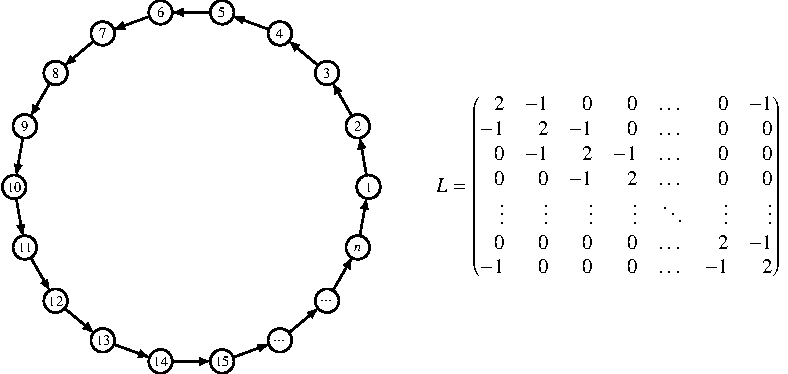
\includegraphics{chapters/70-graphen/images/kreis.pdf}
\caption{Beispiel Graph zur Illustration der verschiedenen Basen auf einem
Graphen.
\label{buch:graphen:fig:kreis}}
\end{figure}
\begin{beispiel}
Wir illustrieren die im folgenden entwickelte Theorie an dem Beispielgraphen
von Abbildung~\ref{buch:graphen:fig:kreis}.
Besonders interessant sind die folgenden Funktionen:
\[
\left.
\begin{aligned}
s_m(k)
&=
\sin\frac{2\pi mk}{n}
\\
c_m(k)
&=
\cos\frac{2\pi mk}{n}
\end{aligned}
\;
\right\}
\quad
\Rightarrow
\quad
e_m(k)
=
e^{2\pi imk/n}
=
c_m(k) + is_m(k).
\]
Das Skalarprodukt dieser Funktionen ist
\[
\langle e_m, e_{m'}\rangle
=
\frac1n
\sum_{k=1}^n
\overline{e^{2\pi i km/n}}
e^{2\pi ikm'/n}
=
\frac1n
\sum_{k=1}^n
e^{\frac{2\pi i}{n}(m'-m)k}
=
\delta_{mm'}
\]
Die Funktionen bilden daher eine Orthonormalbasis des Raums der
Funktionen auf $G$.
Wegen $\overline{e_m} = e_{-m}$ folgt, dass für gerade $n$
die Funktionen
\[
c_0, c_1,s_1,c_2,s_2,\dots c_{\frac{n}2-1},c_{\frac{n}2-1},c_{\frac{n}2}
\]
eine orthonormierte Basis.
\end{beispiel}


Die Laplace-Matrix kann mit der folgenden Definition zu einer linearen
Abbildung auf Funktionen auf dem Graphen gemacht werden.
Sei $f\colon V\to \mathbb{R}$ und $L$ die Laplace-Matrix mit
Matrixelementen $l_{vv'}$ wobei $v,v'\in V$ ist.
Dann definieren wir die Funktion $Lf$ durch
\[
(Lf)(v)
=
\sum_{v'\in V} l_{vv'}f(v').
\]

\subsection{Standardbasis und Eigenbasis
\label{buch:subsection:standardbasis-und-eigenbasis}}
Die einfachste Basis, aus der siche Funktionen auf dem Graphen linear
kombinieren lassen, ist die Standardbasis.
Sie hat für jeden Knoten $v$ des Graphen eine Basisfunktion mit den Werten
\[
e_v\colon V\to\mathbb R:v'\mapsto \begin{cases}
1\qquad&v=v'\\
0\qquad&\text{sonst.}
\end{cases}
\]


\subsection{Wavelet-Basen
\label{buch:subsection:wavelet-basen}}






